\section{Mise en Page Générale}

%-----------------------
\subsection{Titre}

\begin{frame}[fragile]{Titre}
  \begin{itemize}
      \item Informations données dans \lstinline|\author{}|, \lstinline|\date{}| and \lstinline|\title{}| \textbf{avant} le \lstinline|\begin{document}|
      \item Création de la page de titre avec \lstinline|\maketitle| \textbf{après} le \lstinline|\begin{document}|
  \end{itemize}
  \begin{columns}
    \begin{column}{0.5\textwidth}
      \begin{lstlisting}[style=nonumbers,mathescape]
\$\color{blue}{\texttt{subject}}${US Presidential Elections}
\title{FBI Investigations}
\$\color{blue}{\texttt{subtitle}}${Russian interference in the 2016 United States elections}

% Séparer les auteurs avec \and
\author{Donald Trump \and Vladimir Putin}

\date{}               % pas de date
\date{\$\color{blue}{\texttt{today}}$}         % aujourd'hui
\date{8 november 2016}

\begin{document}

\maketitle

\end{document}
      \end{lstlisting}
    \end{column}
    \begin{column}{0.5\textwidth}
  \centering
  \fbox{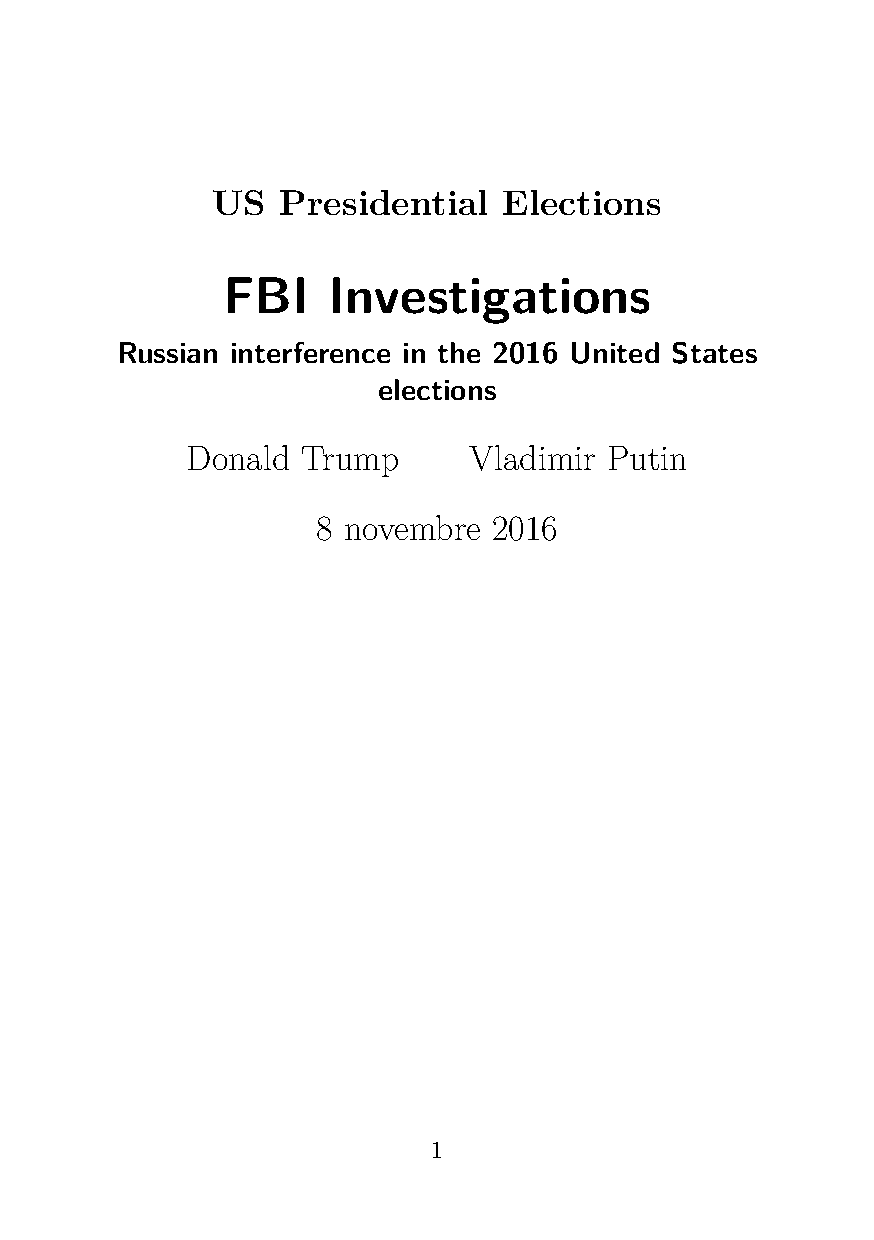
\includegraphics[width=1\textwidth,trim={1.5cm 10cm 1.5cm 1cm},clip]{../build_latex/examples/title/main.pdf}}
    \end{column}
  \end{columns}
\end{frame}

%-----------------------
\subsection{Le Résumé ou Abstract}

\begin{frame}[fragile]{Le résumé ou abstract}
  \begin{itemize}
      \item L'environnement \lstinline|abstract| permet de mettre en page un résumé au début du document.
  \end{itemize}
  \begin{columns}
    \begin{column}{0.5\textwidth}
      \begin{lstlisting}[style=nonumbers]
\begin{document}
...
\begin{abstract}
Voici un résumé succint du contenu
de mon document.
\end{abstract}
...
\end{document}
      \end{lstlisting}
    \end{column}
    \begin{column}{0.5\textwidth}
              \begin{abstract}
                  Voici un résumé succint du contenu de mon document.
              \end{abstract}
    \end{column}
  \end{columns}
\end{frame}

%-----------------------
\subsection{La Table des Matières}

\begin{frame}[fragile]{Table des matières}
  \begin{itemize}
      \item La commande \lstinline|\tableofcontents| suffit pour générer toute la table des matières dynamiquement à partir de vos sections, sous-sections etc.
  \end{itemize}
  \begin{columns}
    \begin{column}{0.6\textwidth}
      \begin{lstlisting}[style=nonumbers]
\begin{document}

\tableofcontents % Table des matières

\section{Introduction}
Ceci est mon premier document en \TeX{}

\section{Le vif du sujet}
Le sujet est en or mais pas le vif.

\subsection{Mais quel est le sujet ?}
\LaTeX{}, ce logiciel d'exception !

\end{document}
      \end{lstlisting}
    \end{column}
    \begin{column}{0.4\textwidth}
      \begin{center}
        \fbox{\includegraphics[width=0.9\textwidth]{table.png}}
      \end{center}
    \end{column}
  \end{columns}
\end{frame}

%-----------------------
\subsection{Listes}

\begin{frame}[fragile]
  \frametitle{Listes}
  \begin{itemize}
    \item Pour faire des listes à puce, utiliser l'environnement \lstinline|itemize|.
    \begin{columns}
      \begin{column}{0.45\textwidth}
        \begin{lstlisting}[style=nonumbers]
\begin{itemize}
  \item Un chat;
  \item une poule;
  \item un chien.
\end{itemize}
        \end{lstlisting}
      \end{column}
      \begin{column}{0.45\textwidth}
        \begin{itemize}
          \item Un chat;
          \item une poule;
          \item un chien.
        \end{itemize}
      \end{column}
    \end{columns}

    \item Pour faire des listes numerotées, utiliser l'environnement \lstinline|enumerate|.
    \begin{columns}
      \begin{column}{0.45\textwidth}
        \begin{lstlisting}[style=nonumbers]
\begin{enumerate}
  \item Mettez de l'eau.
  \item Chauffer l'eau.
  \item Mettez les pasta.
\end{enumerate}
        \end{lstlisting}
      \end{column}
      \begin{column}{0.45\textwidth}
        \begin{enumerate}
          \item Mettez de l'eau.
          \item Chauffer l'eau.
          \item Mettez les pâtes.
        \end{enumerate}
      \end{column}
    \end{columns}
  \end{itemize}
\end{frame}

%-----------------------
\subsection{Exercice 1}

\begin{frame}[fragile]{Premier exercice}
  \framesubtitle{(Utilisez la classe \texttt{scrartcl})}
  \begin{center}
      \fbox{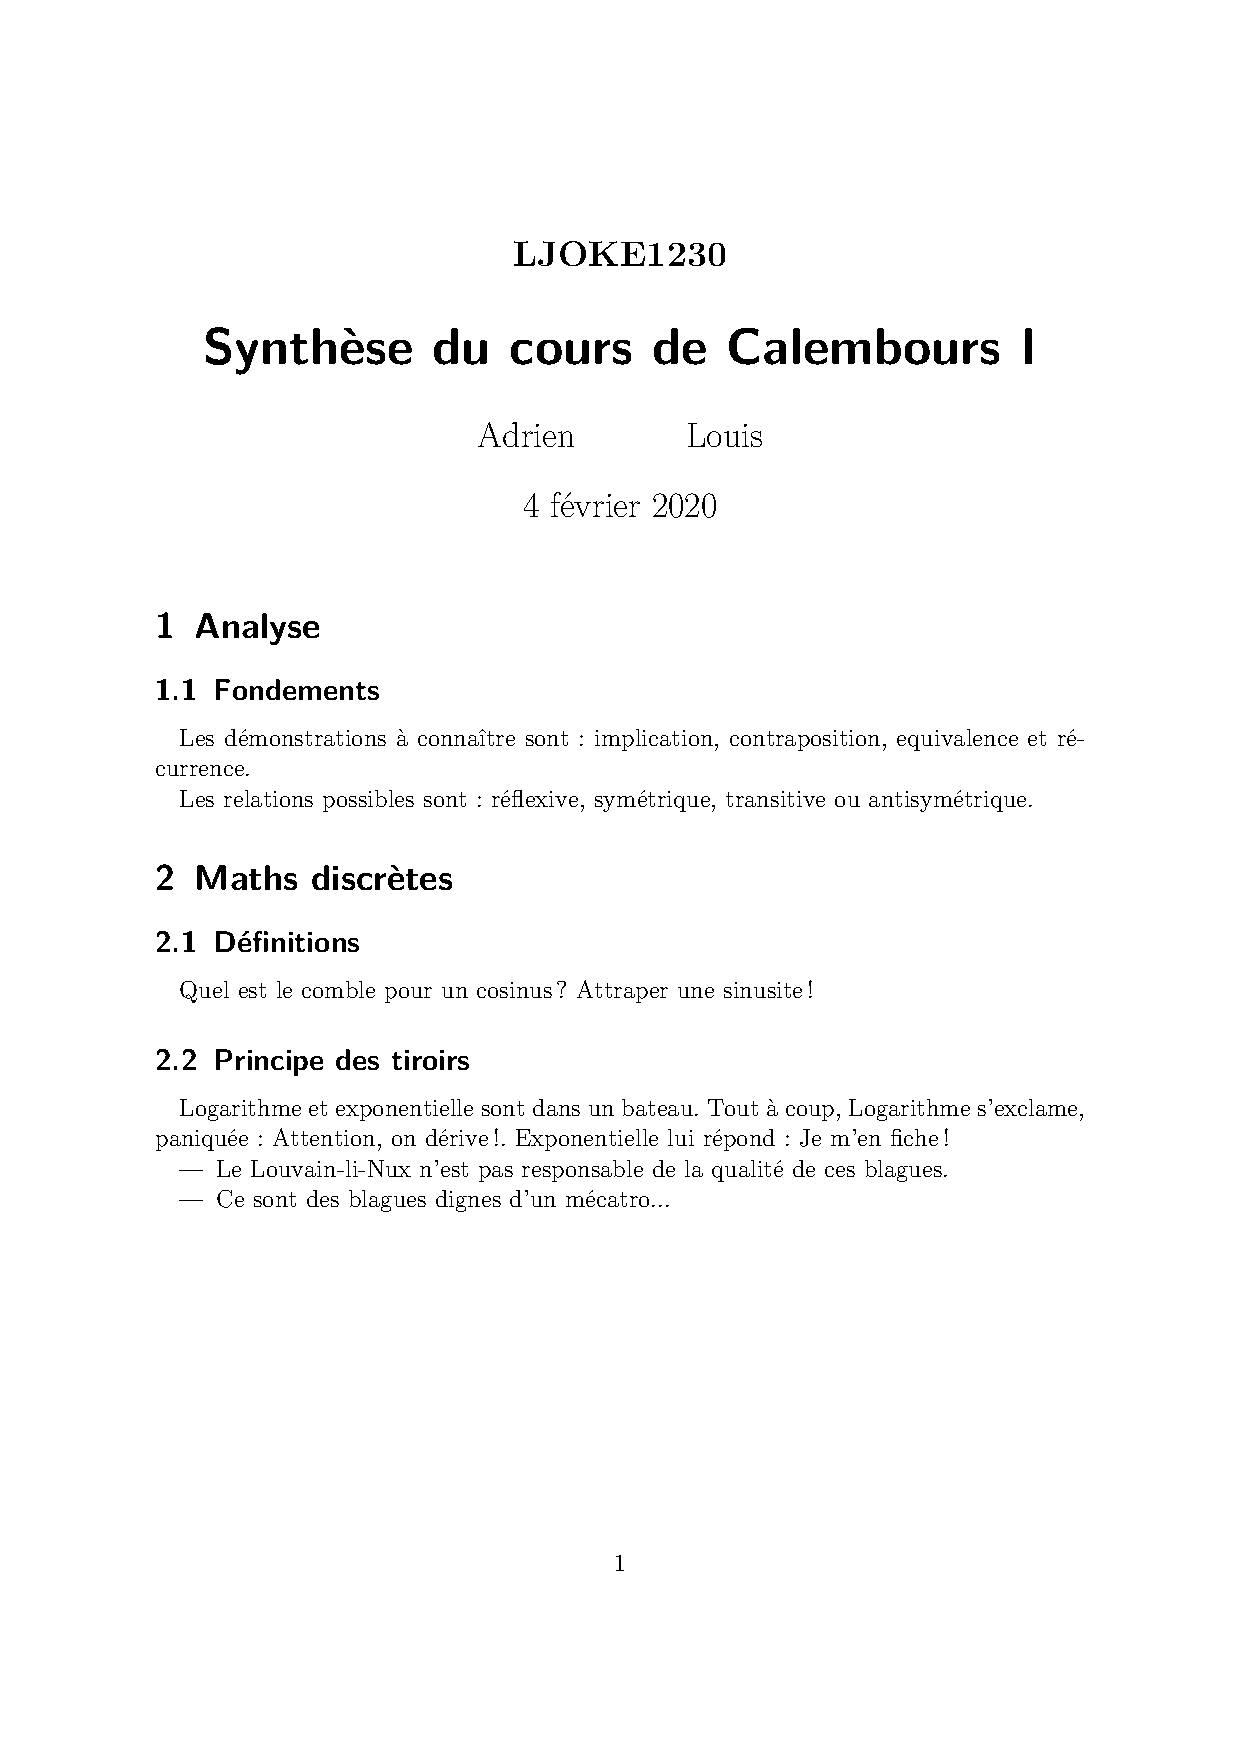
\includegraphics[height=7cm,trim={1.5cm 8cm 1.5cm 3cm},clip]{../build_latex/exercices/1/main.pdf}}
  \end{center}
\end{frame}

\begin{frame}[fragile]{Premier exercice (solution)}
  \begin{center}
  Lien Overleaf de la solution du premier exercice \url{https://www.overleaf.com/read/cgsxdzhjrknb}
  \end{center}
\end{frame}

%-----------------------
\subsection{Notes de Bas de Page}

\begin{frame}[fragile]
  \frametitle{Notes de bas de page}
  La commande \lstinline|\footnote{}| permet d'ajouter une note de bas de page:
  \begin{lstlisting}[style=nonumbers]
It's the ship that made the Kessel\footnote{Kessel is a planet in the Outer Rim} run in less than twelve parsecs\footnote{Whatever that means...}.

She's fast enough for you, old man.
  \end{lstlisting}
  \begin{minipage}{\textwidth}
    It's the ship that made the Kessel\footnote{Kessel is a planet in the Outer Rim} run in less than twelve parsecs\footnote{Whatever that means...}.

    She's fast enough for you, old man.
  \end{minipage}
\end{frame}

%-----------------------
\subsection{Polices d'Écriture}

\begin{frame}[fragile]{Changer la fonte de la police}
  \begin{itemize}
      \item Mise en emphase:
      \begin{center}
      \begin{tabular}{ll}
      \lstinline|\emph{Emphase}| & Mise en \emph{emphase} du texte
      \end{tabular}
      \end{center}
  \item Style de police
  \begin{center}
  \begin{tabular}{ll}
  \lstinline|\textbf{Gras}| & \textbf{Gras} \\
  \lstinline|\textit{Italique}| & \textsl{Italique} \\
  \lstinline|\textsc{Petites majuscules}| & \textsc{Petites majuscules} \\
  \lstinline|\texttt{Machine à écrire}| & \texttt{Machine à écrire} \\
  \lstinline|\textrm{Serif (par défaut)}| & \textrm{Serif (par défaut)}
  \end{tabular}
  \end{center}
  \end{itemize}
\end{frame}

%-----------------------
\subsection{Divers}

\begin{frame}[fragile]{Divers}
  \frametitle{Divers}
  \begin{itemize}
  \item Caractères spéciaux utilisés par \LaTeX

  \begin{tabular}{cccccccccc}
  \lstinline|\$| & \lstinline|\&| & \lstinline|\%| & \lstinline|\#| & \lstinline|\_| & \lstinline|\{| & \lstinline|\}| & \lstinline|\~{}| & \lstinline|\^{}| & \lstinline|\textbackslash| \\
  \$ & \& & \% & \# & \_ & \{ & \} & \~{} & \^{} & \textbackslash
  \end{tabular}

  \item Tirets
   \begin{tabular}{llp{0.5\textwidth}}
     \lstinline|-| & court & Jean-Patrick\\
     \lstinline|--| & moyen ou semi-cadratin & 1984--2015\\
     \lstinline|---| & cadratin & le \LaTeX{} --- c'est chouette --- a été créé par Leslie Lamport\\
   \end{tabular}

  \item Autres caractères (attention, certains nécessitent la présence du package \texttt{babel (french)})
    \begin{itemize}
        \item \lstinline|M\up{me}| pour M\up{me}
        \item \lstinline|1\ier{} 2\ieme{}| pour 1\ier{} et 2\ieme{}
        \item \lstinline|\no \No| pour \no et \No
    \end{itemize}
  \end{itemize}
\end{frame}
